\documentclass[10pt]{beamer}

\usepackage[utf8]{inputenc}
\usepackage[T1]{fontenc}
\usepackage{tgheros}
\usepackage{graphicx}
\usepackage{booktabs}
\usepackage{tabularx}
\usepackage{array}
\usepackage{mathtools}
\usepackage{amsmath}
\usepackage{amssymb}
\usepackage{ragged2e}
\usepackage{adjustbox}
\usepackage{tikz}
\usetikzlibrary{positioning,arrows.meta,fit,backgrounds}
\usepackage{hyperref}

\usetheme{CambridgeUS}
\usecolortheme{dolphin}
\renewcommand{\familydefault}{\sfdefault}
\renewcommand{\arraystretch}{1.12}

% University of Ottawa brand colors
\definecolor{uOttawaPrimary}{HTML}{8F001A}
\definecolor{uOttawaSecondary}{HTML}{9C1C30}
\definecolor{uOttawaLight}{RGB}{245,235,237}
\definecolor{uOttawaGray}{HTML}{4F4F4F}

\setbeamercolor*{palette primary}{bg=uOttawaLight, fg=uOttawaPrimary}
\setbeamercolor*{palette secondary}{bg=uOttawaSecondary, fg=white}
\setbeamercolor*{palette tertiary}{bg=uOttawaPrimary, fg=white}
\setbeamercolor*{subsection in head/foot}{bg=uOttawaSecondary, fg=white}
\setbeamercolor*{titlelike}{fg=uOttawaPrimary}
\setbeamercolor*{title}{bg=uOttawaPrimary, fg=white}
\setbeamercolor*{frametitle}{bg=uOttawaPrimary, fg=white}
\setbeamercolor*{frametitle right}{bg=uOttawaSecondary, fg=white}
\setbeamercolor*{structure}{fg=uOttawaPrimary}
\setbeamercolor*{item}{fg=uOttawaPrimary}
\setbeamercolor*{caption name}{fg=uOttawaPrimary}
\setbeamercolor*{block title}{bg=uOttawaPrimary, fg=white}
\setbeamercolor*{block body}{bg=uOttawaLight, fg=black}
\setbeamercolor*{alerted text}{fg=uOttawaPrimary}
\usefonttheme{professionalfonts}
\setbeamertemplate{navigation symbols}{}
\setbeamertemplate{footline}[frame number]
\hypersetup{colorlinks=true, urlcolor=uOttawaPrimary, linkcolor=uOttawaPrimary}

\titlegraphic{
\includegraphics[height=0.72cm]{uottawa-logo.eps}}

\setbeamerfont{title}{family=\sffamily,series=\bfseries,size=\Large}
\setbeamerfont{subtitle}{family=\sffamily,size=\normalsize}
\setbeamerfont{author}{family=\sffamily,size=\small}
\setbeamerfont{date}{family=\sffamily,size=\small}
\setbeamerfont{institute}{family=\sffamily,size=\small}
\setbeamerfont{frametitle}{family=\sffamily,series=\bfseries,size=\large}

\title[Personalized Web Agents]{Large Language Models Empowered\\Personalized Web Agents}
\subtitle{CSI5389 Paper Presentation}
\author[S. Cai, E. Sun, Y. Zhang]{Sabrina Cai \and Eric Sun \and Yan Zhang}
\institute[EECS, University of Ottawa]{EECS, University of Ottawa\\
\texttt{\{hcai062, ysun338, Yan.Zhang\}@uOttawa.ca}}
\date[March 10, 2026]{March 10, 2026}

\newcommand{\keypoint}[1]{\textcolor{uOttawaPrimary}{\textbf{#1}}}
\newcommand{\speaker}[1]{\framesubtitle{Presenter: #1}}
\newcommand{\paperasset}[3][0.92\linewidth]{%
  \IfFileExists{#2}{%
    \includegraphics[width=#1]{#2}%
  }{%
    \begin{beamercolorbox}[wd=\linewidth,sep=0.9em,rounded=true,shadow=true]{block body}%
      \centering
      {\bfseries Extracted paper figure needed}\\[0.35em]
      {\scriptsize Save the extracted asset as \texttt{\detokenize{#2}}}\\[0.4em]
      {\footnotesize #3}
    \end{beamercolorbox}%
  }%
}

\AtBeginSection[]{
  \begin{frame}[plain]
    \vfill
    \centering
    \begin{beamercolorbox}[sep=10pt,center,shadow=true,rounded=true]{title}
      \usebeamerfont{title}\insertsectionhead\par
    \end{beamercolorbox}
    \vspace{0.8em}
    \begin{minipage}{0.72\linewidth}
      \tableofcontents[currentsection,hideallsubsections]
    \end{minipage}
    \vfill
  \end{frame}
}

\begin{document}

\begin{frame}
  \titlepage
\end{frame}

\begin{frame}{Presentation roadmap}
  \begin{block}{Stage A --- Sabrina}
    \small
    \begin{itemize}
      \item Introduction
      \item Related work
      \item Task formulation
    \end{itemize}
  \end{block}
  \begin{block}{Stage B --- Eric}
    \small
    \begin{itemize}
      \item Benchmark construction
      \item Evaluation
      \item Benchmark analysis
    \end{itemize}
  \end{block}
  \begin{block}{Stage C --- Yan}
    \small
    \begin{itemize}
      \item \textbf{PUMA} framework
      \item Experiments
      \item Conclusion \& future work
    \end{itemize}
  \end{block}
\end{frame}

\section{Background \& Problem Statement}

\begin{frame}{Why do we need personalized web agents?}
  \speaker{Sabrina}
  \begin{columns}[T,onlytextwidth]
    \column{0.58\textwidth}
      \begin{itemize}
        \item Modern web services are powerful but \keypoint{hard to navigate efficiently}.
        \item Existing web agents usually optimize for \keypoint{instruction following}, not for \keypoint{user preference matching}.
        \item Many real requests are \textit{underspecified}:\
        \begin{itemize}
          \item ``Find me a backpack''
          \item ``Recommend a product for my kitchen''
          \item ``Write a review for this item''
        \end{itemize}
        \item These tasks only make sense when the agent also knows the user's:
        \begin{itemize}
          \item purchase history,
          \item budget and brand preferences,
          \item writing tone and review habits.
        \end{itemize}
      \end{itemize}
    \column{0.40\textwidth}
      \begin{block}{Paper thesis}
        \small
        Better web agents must combine:
        \begin{enumerate}
          \item the current instruction,
          \item personalized user data,
          \item and the right web action.
        \end{enumerate}
      \end{block}
      \begin{block}{Key shift}
        \small
        From \textbf{generic automation} to \textbf{user-aware automation}.
      \end{block}
  \end{columns}
\end{frame}

\begin{frame}{From traditional agents to personalized agents}
  \speaker{Sabrina}
  \begin{columns}[T,onlytextwidth]
    \column{0.56\textwidth}
      \paperasset{figures/figure-1.png}{Figure 1: Comparison between traditional Web agents and personalized Web agents.}
    \column{0.40\textwidth}
      \begin{block}{Traditional agent}
        \small
        \begin{itemize}
          \item current query only
          \item general instruction following
          \item weak preference awareness
        \end{itemize}
      \end{block}
      \begin{block}{Personalized agent}
        \small
        \begin{itemize}
          \item profile + behavior history
          \item hidden preference inference
          \item personalized action + parameters
        \end{itemize}
      \end{block}
  \end{columns}
  \vspace{0.2em}
  \centering
\end{frame}

\begin{frame}{Related work and the missing bridge}
  \speaker{Sabrina}
  {\scriptsize Retyped from Table 1.\par}
  \vspace{0.35em}

  {\footnotesize
  \renewcommand{\arraystretch}{1.15}
  \begin{tabularx}{\textwidth}{@{}>{\raggedright\arraybackslash}X>{\centering\arraybackslash}p{0.2\textwidth}>{\centering\arraybackslash}p{0.2\textwidth}>{\centering\arraybackslash}p{0.2\textwidth}@{}}
    \toprule
    Benchmark & Interaction & Environment & Personalization \\
    \midrule
    MiniWoB++ & Single-turn & Mobile UI & No \\
    WebShop & Single-turn & Shopping UI & No \\
    WebArena & Single-turn & Web UI & No \\
    WebLINX & Multi-turn & Web UI & No \\
    ChatShop & Multi-turn & Web function & No \\
    \textbf{PersonalWAB} & \textbf{Single + Multi} & \textbf{Web function} & \textbf{Yes} \\
    \bottomrule
  \end{tabularx}\par}

  \vspace{0.5em}
  \small
  \begin{itemize}
    \item \keypoint{Web-agent benchmarks} study browsing, navigation, or shopping.
    \item \keypoint{Personalized LLM work} studies dialogue, content generation, and recommendation.
    \item The missing piece is \textbf{personalized function execution}: can an agent select the right web action and fill it with user-specific parameters?
  \end{itemize}
\end{frame}

\begin{frame}{Task formulation: what exactly is the agent solving?}
  \speaker{Sabrina}
  \begin{block}{Personalized web interaction}
    \scriptsize
    Given a user instruction $i$, a user profile $P_u$, a behavior memory $M_u$, and callable web functions $\mathcal{F}$, the agent must output
    \[
      f \in \mathcal{F}, \qquad \mathbf{p} = \text{personalized parameters},
    \]
    so the returned result matches both the user's \textbf{explicit request} and \textbf{implicit preferences}.
  \end{block}
  \begin{columns}[T,onlytextwidth]
    \column{0.49\textwidth}
      \begin{block}{Inputs}
        \small
        \begin{itemize}\itemsep0.15em
          \item User instruction
          \item Simulated user profile
          \item Historical web behaviors
          \item Available web functions
        \end{itemize}
      \end{block}
    \column{0.49\textwidth}
      \begin{block}{Outputs}
        \small
        \begin{itemize}\itemsep0.15em
          \item Correct function selection
          \item Correct parameter format
          \item Personalized result or response
        \end{itemize}
      \end{block}
  \end{columns}
  \begin{alertblock}{Why this is harder than standard web agents}
    \scriptsize Two difficulties must be solved together: choosing a valid action and inferring preferences that are often \textbf{not explicitly stated}.
  \end{alertblock}
\end{frame}

\begin{frame}{Main contributions of the paper}
  \speaker{Sabrina}
  \begin{enumerate}
    \item \textbf{New task:} personalized web agents as a formal research problem.
    \item \textbf{New benchmark:} \textbf{PersonalWAB}, covering personalized search, recommendation, and review generation.
    \item \textbf{New method:} \textbf{PUMA} (Personalized User Memory-enhanced Alignment).
    \item \textbf{Main result:} retrieving user history improves action selection and result quality, especially for \textbf{underspecified} instructions.
  \end{enumerate}
  \vspace{0.4em}
  \begin{block}{Take-home message}
    \small Personalization is both a \textbf{memory retrieval} problem and an \textbf{alignment} problem.
  \end{block}
\end{frame}

\section{Benchmark Construction \& Analysis}

\begin{frame}{RL-style view: priors, environment, and algorithm}
  \speaker{Eric}
  \centering
  \begin{block}{Why this benchmark matters beyond this paper}
    \footnotesize
    In an RL-style view, agent capability comes from
    $\text{performance} \approx \textbf{priors} + \textbf{environment} + \textbf{algorithm}$.
    This paper contributes to \emph{all three}, and especially clarifies the \textbf{environment} for personalized web agents.
  \end{block}

  \vspace{0.05em}
  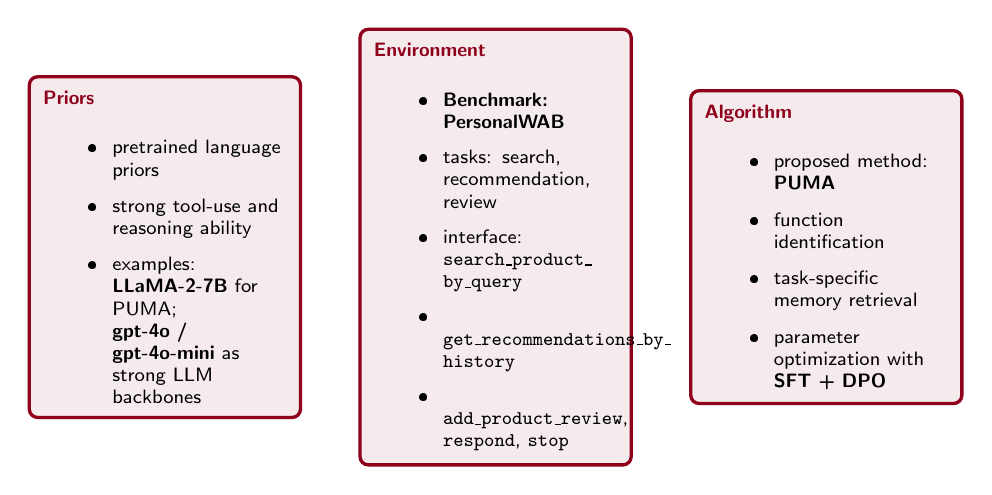
\begin{tikzpicture}[
    font=\scriptsize,
    >=Latex,
    pillar/.style={rounded corners=3pt, draw=uOttawaPrimary, fill=uOttawaLight, very thick, align=left, inner sep=5pt, text width=0.255\textwidth},
    plus/.style={font=\Large\bfseries, text=uOttawaPrimary}
  ]
    \node[pillar] (p1) at (-4.2,0.05) {
      {\color{uOttawaPrimary}\bfseries Priors}\\[0.2em]
      \begin{itemize}\itemsep0.15em
        \item pretrained language priors
        \item strong tool-use and reasoning ability
        \item examples: \textbf{LLaMA-2-7B} for PUMA; \\
        \textbf{gpt-4o / gpt-4o-mini} as strong LLM backbones
      \end{itemize}
    };

    \node[plus] (plus1) at (-1.48,0.05) {+};

    \node[pillar] (p2) at (0,0.05) {
      {\color{uOttawaPrimary}\bfseries Environment}\\[0.2em]
      \begin{itemize}\itemsep0.1em
        \item \textbf{Benchmark: PersonalWAB}
        \item tasks: search, recommendation, review
        \item interface: \texttt{search\_product\_}\\
        \texttt{by\_query}
        \item \texttt{get\_recommendations\_by\_}\\
        \texttt{history}
        \item \texttt{add\_product\_review}, \texttt{respond}, \texttt{stop}
      \end{itemize}
    };

    \node[plus] (plus2) at (2.72,0.05) {+};

    \node[pillar] (p3) at (4.2,0.05) {
      {\color{uOttawaPrimary}\bfseries Algorithm}\\[0.2em]
      \begin{itemize}\itemsep0.15em
        \item proposed method: \textbf{PUMA}
        \item function identification
        \item task-specific memory retrieval
        \item parameter optimization with \textbf{SFT + DPO}
      \end{itemize}
    };
  \end{tikzpicture}

\end{frame}

\begin{frame}{PersonalWAB: benchmark construction pipeline}
  \speaker{Eric}
  \centering
  \paperasset[\linewidth]{figures/figure-2.png}{Figure 2: Overall pipeline for constructing PersonalWAB benchmark with a real example for recommendation instruction.}
  \vspace{0.5em}
  \begin{block}{How to read the pipeline}
    \small
    \begin{itemize}
      \item Built from \textbf{Amazon Review} data rather than expensive real-time user studies.
      \item Pipeline has three main stages: personalized data construction, instruction creation, and web environment implementation.
      \item The objective is to isolate the \textbf{personalization challenge} in a controlled setting.
    \end{itemize}
  \end{block}
\end{frame}

\begin{frame}{How the benchmark data is built}
  \speaker{Eric}
  \begin{columns}[T,onlytextwidth]
    \column{0.54\textwidth}
      \begin{itemize}
        \item \textbf{1,000 users} are sampled from Amazon Reviews.
        \item Five product categories:
        \begin{itemize}
          \item Electronics
          \item Home and Kitchen
          \item Grocery and Gourmet Food
          \item Clothing, Shoes, and Jewelry
          \item Health and Household
        \end{itemize}
        \item Chronological split per user:
        \begin{itemize}
          \item 80\% history
          \item 10\% train
          \item 10\% test
        \end{itemize}
      \end{itemize}
    \column{0.44\textwidth}
      \begin{block}{User profile dimensions}
        \small
        \begin{itemize}
          \item basic info
          \item shopping preferences
          \item behavioral tendencies
          \item tone and style
          \item item references
          \item focus aspects in reviews
        \end{itemize}
      \end{block}
  \end{columns}
\end{frame}

\begin{frame}{Three tasks and a function-based web environment}
  \speaker{Eric}
  \begin{columns}[T,onlytextwidth]
    \column{0.50\textwidth}
      \begin{block}{Task families}
        \small
        \begin{itemize}
          \item \textbf{Search}: produce a personalized query
          \item \textbf{Recommendation}: choose relevant products from history
          \item \textbf{Review}: generate a personalized review text
        \end{itemize}
      \end{block}
      \begin{block}{Why functions instead of full GUIs?}
        \small
        The authors abstract away noisy web interfaces so evaluation focuses on whether the agent chooses the \textbf{right personalized action}.
      \end{block}
    \column{0.48\textwidth}
      \begin{block}{Implemented web functions}
        \small
        \begin{itemize}
          \item \texttt{search\_product\_by\_query}
          \item \texttt{get\_recommendations\_by\_history}
          \item \texttt{add\_product\_review}
          \item \texttt{respond}
          \item \texttt{stop}
        \end{itemize}
      \end{block}
      \begin{alertblock}{Key design choice}
        \small The benchmark tests \textbf{personalization ability}, not browser navigation skill.
      \end{alertblock}
  \end{columns}
\end{frame}

\begin{frame}{Evaluation protocol}
  \speaker{Eric}
  \begin{columns}[T,onlytextwidth]
    \column{0.51\textwidth}
      \begin{block}{Two tracks}
        \small
        \begin{itemize}
          \item \textbf{Single-turn}: one chance to act
          \item \textbf{Multi-turn}: agent can ask/respond and receive simulator feedback
        \end{itemize}
      \end{block}
      \begin{block}{Metrics}
        \small
        \begin{itemize}
          \item \textbf{Function accuracy}: right function + valid parameter format
          \item \textbf{Result accuracy}: quality of returned result
          \item \textbf{Average steps}: multi-turn efficiency
        \end{itemize}
      \end{block}
    \column{0.47\textwidth}
      \begin{block}{Search / recommendation result accuracy}
        \small
        \[
        \mathrm{ResAcc}=
        \begin{cases}
          1-\dfrac{r-1}{10}, & r \le 10,\\[0.4em]
          0, & r > 10.
        \end{cases}
        \]
        \vspace{-0.8em}
        \begin{itemize}
          \item $r$ is the rank of the target product in the returned list.
          \item For review generation, the paper instead uses sentence-level similarity.
        \end{itemize}
      \end{block}
  \end{columns}
\end{frame}

\begin{frame}{What does PersonalWAB contain?}
  \speaker{Eric}
  \centering
  \scriptsize
  \begin{tabular}{@{}>{\raggedright\arraybackslash}p{0.22\linewidth}>{\centering\arraybackslash}p{0.20\linewidth}>{\centering\arraybackslash}p{0.20\linewidth}>{\centering\arraybackslash}p{0.20\linewidth}@{}}
    \toprule
    Group & Statistic & Train & Test \\
    \midrule
    User & \# Users & 939 & 1,000 \\
    User & Avg. profile tokens & 247 & --- \\
    User & Avg. behavior length & 32 & 38 \\
    User & Avg. behavior tokens & 7,597 & 9,270 \\
    Instruction & \# Instructions & 6,896 & 2,174 \\
    Instruction & Avg. instruction tokens & 46 & 45 \\
    Product & \# Products & 8,236 & --- \\
    Product & Avg. product tokens & 665 & --- \\
    \bottomrule
  \end{tabular}
  \vspace{0.5em}
  \begin{block}{Interpretation}
    \small The benchmark is not tiny: each test instance combines a user profile, long behavior history, task instruction, product space, and callable tools.
  \end{block}
\end{frame}

\begin{frame}{Benchmark analysis: diversity of users and instructions}
  \speaker{Eric}
  \begin{columns}[T,onlytextwidth]
    \column{0.49\textwidth}
      \paperasset[\linewidth]{figures/figure-3.png}{Figure 3: Distribution of users by gender, age, and occupation.}
    \column{0.49\textwidth}
      \paperasset[\linewidth]{figures/figure-4.png}{Figure 4: (a) Distribution of behaviors by Price Sensitivity, Diversity Preference, and Interaction Complexity; (b) Statistics of the instructions on different tasks.}
  \end{columns}
  \vspace{0.4em}
  \begin{block}{Key observations}
    \small
    \begin{itemize}
      \item Profiles cover a \keypoint{wide spread of demographics} and occupations.
      \item Behavioral attributes include price sensitivity, diversity preference, and interaction complexity.
      \item Most users fall into the \textbf{medium} range, but there are enough \textbf{low/high} cases to stress-test personalization.
      \item Recommendation instructions are usually shorter; review instructions are slightly more expressive and detailed.
    \end{itemize}
  \end{block}
\end{frame}

\begin{frame}{Benchmark analysis: are the generated profiles believable?}
  \speaker{Eric}
  \centering
  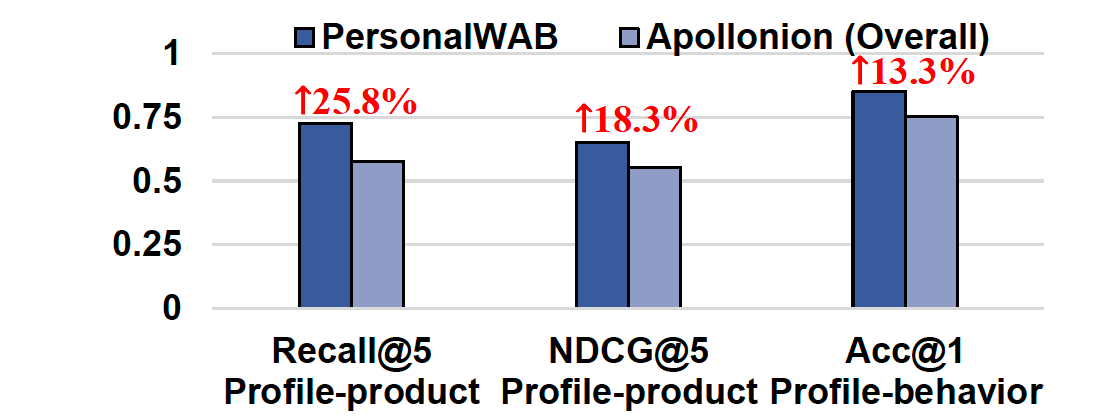
\includegraphics[width=\linewidth,height=0.34\textheight,keepaspectratio]{figures/figure-5.png}
  \vspace{0.25em}
  \begin{columns}[T,onlytextwidth]
    \column{0.48\textwidth}
      \begin{block}{Profile consistency evaluation}
        \small
        The paper checks whether a generated profile actually matches:
        \begin{itemize}
          \item the user's past behaviors,
          \item the user's likely interesting products.
        \end{itemize}
      \end{block}
    \column{0.48\textwidth}
      \begin{alertblock}{Observed gain}
        \small
        PersonalWAB improves over Apollonion by roughly:
        \begin{itemize}
          \item \textbf{+25.8\%} on Recall@5,
          \item \textbf{+18.3\%} on NDCG@5,
          \item \textbf{+13.3\%} on Acc@1.
        \end{itemize}
      \end{alertblock}
  \end{columns}
\end{frame}

\begin{frame}{Benchmark strengths and limitations}
  \speaker{Eric}
  \begin{columns}[T,onlytextwidth]
    \column{0.49\textwidth}
      \begin{block}{Why this benchmark matters}
        \small
        \begin{itemize}
          \item first benchmark centered on \textbf{personalized web-agent behavior}
          \item evaluates both \textbf{single-turn} and \textbf{multi-turn} interaction
          \item separates \textbf{function choice} from \textbf{parameter quality}
        \end{itemize}
      \end{block}
    \column{0.49\textwidth}
      \begin{block}{What it still abstracts away}
        \small
        \begin{itemize}
          \item e-commerce only
          \item function abstraction instead of messy real websites
          \item simulated profiles and user simulator instead of real deployment
        \end{itemize}
      \end{block}
      \begin{alertblock}{Evaluation takeaway}
        \small PersonalWAB is a \textbf{clean testbed} for personalization, but not the full web.
      \end{alertblock}
  \end{columns}
\end{frame}

\section{PUMA, Experiments \& Conclusion}

\begin{frame}{PUMA: the main method idea}
  \speaker{Yan}
  \centering
  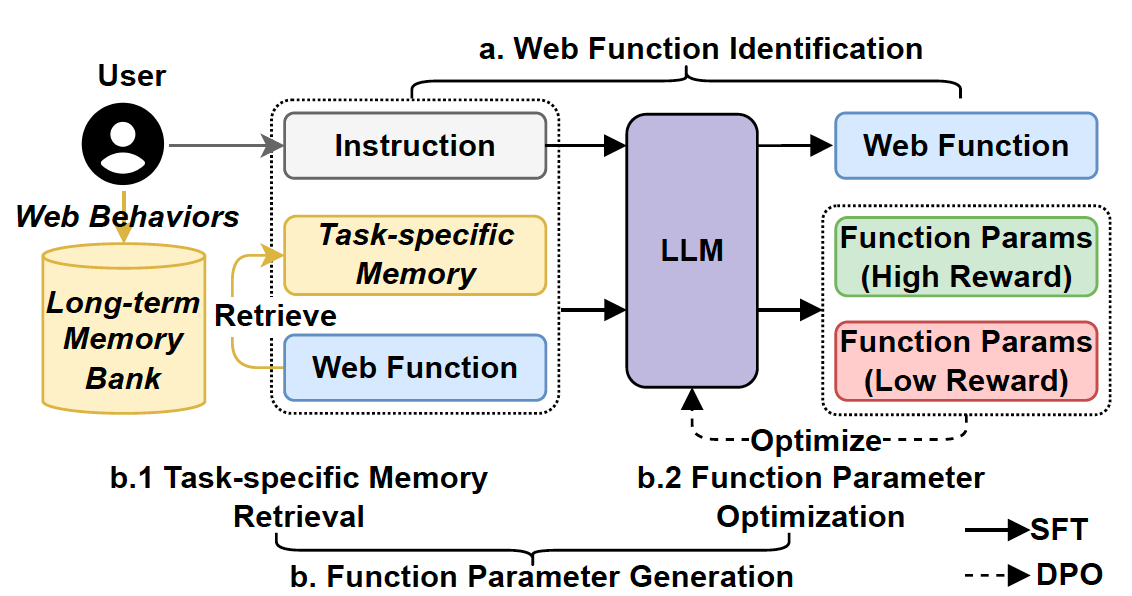
\includegraphics[width=\linewidth,height=0.33\textheight,keepaspectratio]{figures/figure-6.png}
  \vspace{0.25em}
  \begin{columns}[T,onlytextwidth]
    \column{0.48\textwidth}
      \begin{block}{Personalized User Memory-enhanced Alignment}
        \small
        \textbf{PUMA} turns personalization into a two-stage pipeline:
        \begin{enumerate}
          \item identify the right web function,
          \item generate the most user-aligned function parameters.
        \end{enumerate}
      \end{block}
    \column{0.48\textwidth}
      \begin{block}{Method intuition}
        \small
        \begin{itemize}
          \item retrieve the \textbf{right slice} of long-term memory,
          \item then align parameter generation with user preference.
        \end{itemize}
      \end{block}
  \end{columns}
\end{frame}

\begin{frame}{Task-specific memory retrieval}
  \speaker{Yan}
  \begin{columns}[T,onlytextwidth]
    \column{0.52\textwidth}
      \begin{block}{Long-term memory bank}
        \small
        For each user, PUMA stores historical purchases, product metadata, ratings, and reviews.
      \end{block}
      \begin{block}{Retrieval strategy}
        \small
        For a new instruction, it retrieves the \textbf{Top-K} most relevant behaviors and then extracts features matched to the chosen function.
      \end{block}
    \column{0.45\textwidth}
      \begin{block}{Equation (2)}
        \scriptsize
        \[
          \begin{aligned}
            M_i &= \mathrm{Extract}\!\bigl(\mathrm{TopK}(M, \\
            &\qquad \mathrm{sim}(i,m_j), K), f\bigr)
          \end{aligned}
        \]
        \vspace{-0.7em}
        \begin{itemize}\itemsep0.15em
          \item $M$: long-term memory bank
          \item $i$: current instruction
          \item $f$: identified web function
        \end{itemize}
      \end{block}
  \end{columns}
\end{frame}

\begin{frame}{Function parameter optimization: SFT + DPO}
  \speaker{Yan}
  \begin{columns}[T,onlytextwidth]
    \column{0.58\textwidth}
      \begin{block}{Stage 1: supervised fine-tuning}
        \small
        Pseudo-labels are built heuristically:
        \begin{itemize}\itemsep0.2em
          \item search: textual query
          \item recommendation: recent product IDs from relevant category
          \item review: actual review text
        \end{itemize}
      \end{block}
    \column{0.38\textwidth}
      \begin{block}{Preference-pair dataset}
        \small
        \[
          \mathcal{D}_{\mathrm{DPO}} = \{(p_i^{b}, p_i^{w}, x_i)\}_{i=1}^{n}
        \]
        Best and worst parameter candidates are chosen by result accuracy.
      \end{block}
  \end{columns}
  \begin{alertblock}{Why Stage 1 matters}
    \small SFT gives the model a reasonable initialization before preference-based optimization.
  \end{alertblock}
\end{frame}

\begin{frame}{Function parameter optimization: Stage 2 with DPO}
  \speaker{Yan}
  \begin{block}{Stage 2: DPO}
    \tiny
    \[
    \begin{aligned}
      \mathcal{L}_{\mathrm{DPO}} = -\mathbb{E}\Bigg[\log \sigma\Bigg(&\beta \log \frac{\pi_{\theta}(p^{b}\mid x)}{\pi_{\mathrm{ref}}(p^{b}\mid x)} \\
      &- \beta \log \frac{\pi_{\theta}(p^{w}\mid x)}{\pi_{\mathrm{ref}}(p^{w}\mid x)}\Bigg)\Bigg]
    \end{aligned}
    \]
    \vspace{-0.9em}
    {\small
    \begin{itemize}\itemsep0.25em
      \item reward better parameters,
      \item suppress worse parameters,
      \item align outputs with user preference.
    \end{itemize}
    }
  \end{block}
  \begin{block}{Intuition}
    \small DPO pushes the model toward parameter choices that lead to better personalized outcomes without requiring an explicit reward model at deployment time.
  \end{block}
\end{frame}

\begin{frame}{Single-turn results: PUMA leads on overall personalization}
  \speaker{Yan}
  \scriptsize
  \begin{adjustbox}{max width=\linewidth}
  \begin{tabular}{@{}lcccccccc@{}}
    \toprule
    & \multicolumn{2}{c}{Search} & \multicolumn{2}{c}{Recommendation} & \multicolumn{2}{c}{Review} & \multicolumn{2}{c}{Overall} \\
    Method & F. Acc. & Res Acc & F. Acc. & Res Acc & F. Acc. & Res Acc & F. Acc. & Res Acc \\
    \midrule
    No Memory (gpt-4o) & 1.000 & 0.647 & 0.092 & 0.000 & 1.000 & 0.444 & 0.684 & 0.355 \\
    Random Memory (gpt-4o) & 0.974 & 0.640 & 0.296 & 0.018 & 0.996 & 0.442 & 0.745 & 0.357 \\
    Last Memory (gpt-4o) & 0.937 & 0.626 & 0.432 & 0.028 & 1.000 & 0.442 & 0.782 & 0.357 \\
    Relevant Memory (gpt-4o) & 0.928 & 0.622 & 0.492 & 0.030 & 1.000 & 0.443 & 0.800 & 0.356 \\
    ReAct (gpt-4o) & 0.903 & 0.605 & 0.560 & 0.027 & 0.996 & 0.444 & 0.815 & 0.350 \\
    RecMind (gpt-4o) & 0.981 & 0.645 & 0.226 & 0.017 & 0.990 & 0.442 & 0.721 & 0.359 \\
    PUMA (gpt-4o) & 1.000 & 0.649 & 0.939 & 0.048 & 1.000 & 0.449 & 0.979 & 0.373 \\
    \textbf{PUMA (LLaMA-7B)} & \textbf{0.996} & \textbf{0.652} & \textbf{0.987} & \textbf{0.054} & \textbf{1.000} & \textbf{0.538} & \textbf{0.994} & \textbf{0.406} \\
    \bottomrule
  \end{tabular}
  \end{adjustbox}
  \vspace{0.5em}
  \begin{alertblock}{Key takeaway}
    \small The biggest improvement is in \textbf{recommendation function accuracy}, where personalization is most needed and generic tool-calling is not enough.
  \end{alertblock}
\end{frame}

\begin{frame}{Multi-turn results: stronger accuracy with controlled interaction}
  \speaker{Yan}
  \scriptsize
  \begin{adjustbox}{max width=\linewidth}
  \begin{tabular}{@{}lccc|ccc|ccc|ccc@{}}
    \toprule
    & \multicolumn{3}{c|}{Search} & \multicolumn{3}{c|}{Recommendation} & \multicolumn{3}{c|}{Review} & \multicolumn{3}{c}{Overall} \\
    Method & F. & R. & Steps & F. & R. & Steps & F. & R. & Steps & F. & R. & Steps \\
    \midrule
    No Memory & 0.996 & 0.656 & 2.398 & 0.096 & 0.000 & 2.420 & 1.000 & 0.446 & 2.019 & 0.685 & 0.358 & 2.280 \\
    Random Memory & 0.999 & 0.680 & 4.193 & 0.703 & 0.042 & 4.474 & 1.000 & 0.448 & 2.007 & 0.896 & 0.380 & 3.564 \\
    Last Memory & 0.996 & 0.676 & 4.229 & 0.708 & 0.045 & 4.252 & 1.000 & 0.449 & 2.007 & 0.897 & 0.381 & 3.498 \\
    Relevant Memory & 0.996 & 0.686 & 4.233 & 0.715 & 0.042 & 4.564 & 0.999 & 0.448 & 2.008 & 0.899 & 0.383 & 3.609 \\
    ReAct & 0.996 & 0.674 & 4.657 & 0.218 & 0.013 & 5.468 & 0.974 & 0.448 & 2.129 & 0.718 & 0.369 & 4.098 \\
    Reflexion & 1.000 & 0.686 & 5.406 & 0.281 & 0.014 & 6.145 & 0.976 & 0.449 & 2.145 & 0.741 & 0.373 & 4.579 \\
    RecMind & 0.997 & 0.642 & 6.728 & 0.347 & 0.026 & 6.003 & 0.997 & 0.451 & 2.107 & 0.771 & 0.364 & 4.938 \\
    InteRecAgent & 0.999 & 0.642 & 3.110 & 0.618 & 0.022 & 3.008 & 1.000 & 0.447 & 2.001 & 0.867 & 0.362 & 2.706 \\
    \textbf{PUMA} & \textbf{0.999} & \textbf{0.720} & 5.082 & \textbf{0.984} & \textbf{0.052} & 3.791 & \textbf{1.000} & \textbf{0.453} & 2.002 & \textbf{0.994} & \textbf{0.399} & 3.608 \\
    \bottomrule
  \end{tabular}
  \end{adjustbox}
  \vspace{0.35em}
  \begin{block}{Interpretation}
    \small In multi-turn settings, memory retrieval helps more, but \textbf{PUMA} still achieves the best overall function accuracy and result accuracy.
  \end{block}
\end{frame}

\begin{frame}{Efficiency: better personalization does not have to be slower}
  \speaker{Yan}
  \centering
  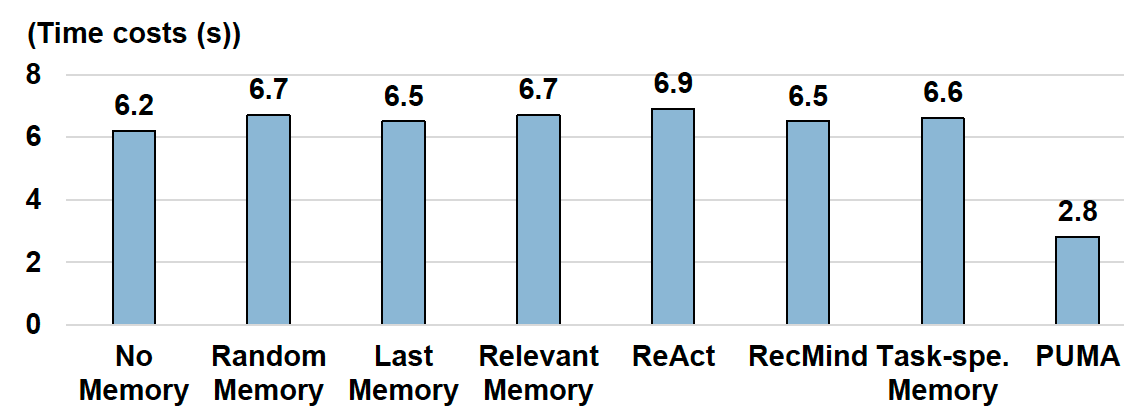
\includegraphics[width=\linewidth,height=0.36\textheight,keepaspectratio]{figures/figure-7.png}
  \vspace{0.25em}
  \begin{columns}[T,onlytextwidth]
    \column{0.48\textwidth}
      \begin{block}{Reported result}
        \small
        In the single-turn track, GPT-based baselines take about \textbf{6.5--6.9 seconds} on average, while \textbf{PUMA} takes about \textbf{2.8 seconds}.
      \end{block}
    \column{0.48\textwidth}
      \begin{alertblock}{Why this matters}
        \small The method is not just more accurate. It is also more practical for deployment where latency matters.
      \end{alertblock}
  \end{columns}
\end{frame}

\begin{frame}{Conclusion: what should we remember?}
  \speaker{Yan}
  \begin{itemize}
    \item The paper formalizes a new setting: \textbf{personalized web agents}.
    \item \textbf{PersonalWAB} provides the first dedicated benchmark for this setting.
    \item \textbf{PUMA} improves performance by combining:
    \begin{itemize}
      \item task-specific memory retrieval,
      \item function identification,
      \item and preference-aligned parameter optimization.
    \end{itemize}
    \item The gains are strongest when the instruction is \textbf{ambiguous or underspecified}.
  \end{itemize}
  \begin{block}{One-sentence summary}
    \small If web agents are meant to act \textit{for users}, they must remember who the users are.
  \end{block}
\end{frame}

\begin{frame}{Limitations and future work}
  \speaker{Yan}
  \begin{columns}[T,onlytextwidth]
    \column{0.49\textwidth}
      \begin{block}{Limitations}
        \small
        \begin{itemize}
          \item restricted to e-commerce
          \item simplified function environment
          \item profile quality depends on stored behavior history
          \item privacy and stale-memory issues remain open
        \end{itemize}
      \end{block}
    \column{0.49\textwidth}
      \begin{block}{Future directions}
        \small
        \begin{itemize}
          \item broader domains and more realistic web environments
          \item dynamic preference updating over time
          \item real user interaction and human-in-the-loop evaluation
          \item fairness, safety, and privacy-aware personalization
        \end{itemize}
      \end{block}
  \end{columns}
  \vspace{0.3em}
  \centering
  {\small Hongru Cai et al., \textit{Large Language Models Empowered Personalized Web Agents}, WWW 2025.}
\end{frame}

\section*{Q\&A}

\begin{frame}[plain]
  \vfill
  \centering
  {\Huge\textcolor{uOttawaPrimary}{Thank you!}}\\[0.6em]
  {\large Questions?}\\[1em]
  \vfill
\end{frame}

\end{document}



